\section{Occupancy Grid Mapping} \label{sec:ogm}
In 1985 Moravec and Elfes \cite{moravec1985high} investigated the use of sonar measurements to map the surroundings of a robot. By gathering sonar measurements from multiple points of view (having several sensors on the robot) and from multiple instances in time, information about the robot's surroundings is accumulated. This information is used to compute the state of each cell within a rasterized 2D \gls{BEV} map of the robot's surroundings is 'occupied', 'unoccupied', or 'unknown' (when there is no sensor data available of that cell), as can be seen in Figure \ref{fig:OGMBEVmoravec}. This is an example of environment representation called an \glsfirst{OGM}. \\

\begin{figure}[h]
	\centering
	\includegraphics[width=0.6\linewidth]{Figures/Occupancy_Grid_Map/The_Two-dimensional_Sonar_map}
	\caption{This image shows an \gls{OGM} of a robot's surrounding environment. The solid lines represent the outline of the room and of the major objects that formed the robot's environment. The large circles in the image are the positions at which the robot performed measurements of its surroundings. The measurements are used to generate the \gls{OGM}, which is a \gls{BEV} raster in which each cell represents the state of an area within the environment. Each cell contains a symbol or white space. Empty areas with a high certainty factor are represented by white space. Empty areas with lower certainty factors are represented by "+" symbols of increasing thickness the lower the certainty. Occupied areas are represented by "x" symbols, and Unknown areas by "." symbols. Image from \cite{moravec1985high}.}
	\label{fig:OGMBEVmoravec}
\end{figure}

Formally, the \gls{OGM} is often represented in a tensor or matrix, $m$, of which each element (cell), $m_{i,j}: i \in [0, M],j \in [0, N]$, represents the occupancy state of an area in the robot's surrounding world. The size of that area depends on the sensor's and grid cell's resolution. The occupancy probability of a cell $m_{i,j}$ is a discrete random variable with two exclusive and exhaustive values, occupied ($O$) and empty ($E$), resulting in equation \ref{eqn:occ_empt} \cite{elfes1989using}. Therefore, knowing only the probability of a cell being occupied $P[m_{i,j} = O]$, which is a number between $0$ and $1$, is enough to determine a cell's state. Given a cell's probability of being occupied, one out of three different states is assigned to that cell based on its probability value. If the probability value is close to $0$, the state is 'Empty', while with a probability value close to $1$ the state is 'Occupied'. If a cell's probability of being occupied is $0.5$, which means that the probability of the cell being empty is also $0.5$, it will be assigned the 'Unknown' state. This is the case for cells corresponding to areas that are unobserved or areas of which conflicting measurements are obtained. \\

\begin{equation} \label{eqn:occ_empt}
	P[m_{i,j} = O] + P[m_{i,j} = E] = 1
\end{equation} 

\hfill \break

For simplicity, the notation $m_{i,j}$ will be used for the case where the cell is occupied $m_{i,j} = O$ and $\neg m_{i,j}$ for the empty state $m_{i,j} = E$.
These state values can be determined in several ways. In section \ref{subsec:prob_OGM}, two probabilistic methods to obtain occupancy state values and generate \glspl{OGM} will be discussed. The first method uses an inverse sensor model and the second uses a forward sensor model. In section \ref{subsec:evid_OGM}, an evidential method for \gls{OGM} generation that uses the \gls{DST} will be discussed. Then, in section \ref{subsec:alt_OGM}, some alternative, less common \gls{OGM} generation methods are briefly discussed.
Besides ways to generate the traditional \gls{OGM} maps that provides information about the cell occupancy, there are extended \gls{OGM} forms that contain more information. Section \ref{subsec:OGM_ext_form} will elaborate on some of those extended forms. Finally, section \ref{subsec:OGM_conclude} concludes this chapter by answering the question: \airquote{\textit{What \gls{OGM} form is most suitable to use in \gls{OGM} prediction methods?}}

%Sources: Environment Perception Using Grid Occupancy, Fusion-2014, using occupancy grids for mobile robot.., probabilistic algorithms in robotics, Learning Occupancy Grids With Forward Sensor Models, Comparative Study of Inverse and Forward Sensor Models


\subsection{Probabilistic Occupancy Grid Mapping} \label{subsec:prob_OGM}
In probabilistic occupancy grid mapping, Bayesian reasoning is used to estimate the state of each cell in the grid. Two processing stages are required to compute the probability of the cell states. First, a sensor measurement is interpreted using a sensor model. Second, the sensor reading is used to update the \gls{OGM} cell's estimates using Bayes' theorem. \cite{elfes1990occupancy} \cite{moras2014evidential}. The two main sensor models that are used to interpret the sensor data are the inverse sensor model \cite{elfes1990occupancy} and the forward sensor model \cite{thrun2003learning}. The selected sensor model affects the assumptions that can be made about the \gls{OGM} and thus affects the performance and computing time of the updated \gls{OGM} cell states. Both sensor models and their implementation of the two processing stages, using Bayes' theorem, will be explained in the next two subsections. In the third subsection, both models will be compared. 

\subsubsection{Bayesian update with inverse sensor model}
The inverse sensor model is formulated according to formula \ref{eqn:inv_sens_dep}. It signifies the conditional probability of the complete occupancy grid map of the environment $m$, given the complete sets of sensor measurements $z_{1:T}$ and corresponding robot poses $x_{1:T}$. This model obtains the map state probability inversely to how the measurements are generated, since measurements are generated \textit{given} the map (environment). \cite{carvalho2013comparative}. 

\begin{equation} \label{eqn:inv_sens_dep}
	p(m|z_{1:T},x_{1:T})
\end{equation}

Given an \gls{OGM}'s size of $M\times N$, there are $2^{M\times N}$ possible grid configurations. As a result, the required computing power needed to estimate a complete \gls{OGM} scales exponentially with the grid size. To tackle this, each cell in the \gls{OGM} is assumed to be conditionally independent given the measurements and the poses, which results in equation \ref{eqn:inv_sens_indep}, where $m_{i,j}$ stands for a single grid cell's occupied state. This computation requires much less computing power. \cite{UoP2021} \cite{carvalho2013comparative}.

\begin{equation} \label{eqn:inv_sens_indep}
	p(m|z_{1:T},x_{1:T}) = \prod_{i,j}^{} p(m_{i,j}|z_{1:T},x_{1:T}) 
\end{equation} 

Also, a static world assumption is made in equation \ref{eqn:inv_static_assum1} which means that a measurement $z$ at time $t$ is conditionally independent from the previous measurements and poses, given the \gls{OGM} cell's state knowledge. Using Bayes' rule, equation \ref{eqn:inv_static_assum2} shows the static assumption in the form that requires the conditional probability of the cell's state given the measurement and pose. This is easier to compute because the cell's state is binary as opposed to the measurement, which can have a much larger range depending on the sensor \cite{carvalho2013comparative}. 

\begin{equation} \label{eqn:inv_static_assum1}
	p(z_t|m_{i,j}, z_{1:t-1}, x_{1:t}) = p(z_t|m_{i,j}, x_t) 
\end{equation}

\begin{equation} \label{eqn:inv_static_assum2}
	p(z_t|m_{i,j}, x_t) = \frac{p(m_{i,j}|z_t, x_t)p(z_t|x_t)}{p(m_{i,j}| x_t)}
\end{equation}

By assigning the estimated \gls{OGM} as the prior estimation for the next time step and given equations \ref{eqn:inv_sens_indep} and \ref{eqn:inv_static_assum2}, Bayes's theorem can be used for every grid cell $m_{i,j}$ to update the \gls{OGM} $m$ recursively every time new sensor data becomes available. This is shown in equation \ref{eqn:inv_sens1} \cite{youtube2020ogm}. 


\begin{equation} \label{eqn:inv_sens1}
	p(m_{i,j}|z_{1:t},x_{1:t}) = \frac{p(z_t|m_{i,j},z_{1:t-1}, x_{1:t}) p(m_{i,j}|z_{1:t-1}, x_{1:t})}{p(z_t| z_{1:t-1}, x_{1:t})} = \frac{p(m_{i,j}|z_t, x_t)p(z_t|x_t) p(m_{i,j}|z_{1:t-1}, x_{1:t})}{p(m_{i,j})p(z_t| z_{1:t-1}, x_{1:t})}
\end{equation}

Because sensors are never ideal, the sensor model transforms a single sensor reading $p(z_t|x_t)$ to a Gaussian range around the reading. This way, a measured cell's neighbors are also given a measurement probability value to consider the inaccuracy of the sensor. Then, equation \ref{eqn:inv_sens1} computes for each (observed) \gls{OGM} cell a probabilistic estimate of its occupancy state.
Unobserved cells are set to have a $p(m_{i,j})$ of $0.5$ and are thus considered 'unknown'.
Afterwards, a threshold is set which determines at what probability a grid cell is considered occupied (Figure \ref{fig:OGMwthresh}), a two-dimensional grid map can be created that can be used for purposes such as motion planning and environment interpretation (Figure \ref{fig:OGMBEVmoravec}). \\	


\begin{figure}[h]
	\centering
	\begin{subfigure}[t]{0.4\linewidth}
		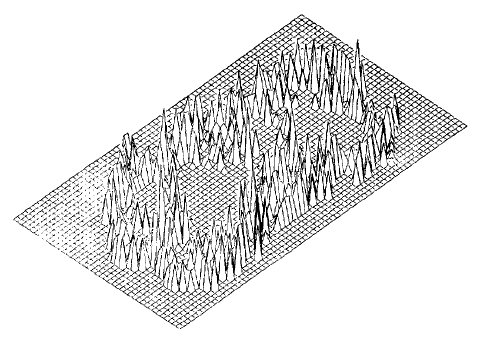
\includegraphics[width=\linewidth]{Figures/Occupancy_Grid_Map/Occupied_Areas_in_Map}
		\caption{This figure shows the occupied areas in the map where the height of the peaks shows the occupancy certainty factors.\cite{moravec1985high}}
		\label{fig:OGMwothresh}
	\end{subfigure} \hspace{0.1\textwidth}
	\begin{subfigure}[t]{0.4\linewidth}
		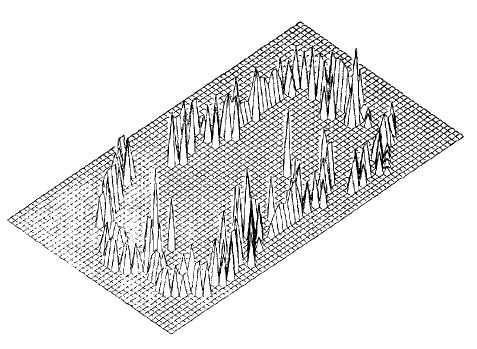
\includegraphics[width=\linewidth]{Figures/Occupancy_Grid_Map/Occupied_Areas_in_Map_after_Thresholding}
		\caption{This figure shows the occupied areas in the map after thresholding the occupancy certainty factors.\cite{moravec1985high}}
		\label{fig:OGMwthresh}
	\end{subfigure}
	\caption{Thresholding of the occupancy grid map data.}
	\label{fig:OGMw-wothresh}
\end{figure}


\subsubsection{Bayesian update with forward sensor model}
The forward sensor model is formulated in formula \ref{eqn:for_sens}. When comparing to the inverse sensor model, this model also makes the static world assumption (i.e. a measurement is conditionally independent from the previous measurements and poses), but does not assume that the grid cell's are conditionally independent. It is a generative model that is modeled as a likelihood. Given the world that is represented by the \gls{OGM} $m$, and the complete set of poses $x_{1:T}$, this formula would give the most likely set of sensor measurements $z_{1:T}$ \cite{carvalho2013comparative}.

\begin{equation} \label{eqn:for_sens}
	p(z_{1:T}|m,x_{1:T})
\end{equation}

To find the \gls{OGM}, the likelihood formula \ref{eqn:for_sens} needs to be maximized by iteratively adjusting $m$. To do so, a reliable sensor model needs to be made.
Not all measurements are caused by obstacles, some are erroneously made. Therefore, it is assumed that all sensor measurements, $z$, can be subdivided into the following three cases to model the sensor. \cite{thrun2003learning} \cite{carvalho2013comparative}.  

\begin{enumerate}
	\item \textbf{Non-random:} A non-random measurement is caused by an obstacle that lies within the sensor's range.
	\item \textbf{Random:} A random measurement covers the remaining causes of a sensor measurement such as specular reflections or false positives.
	\item \textbf{Maximum reading:} When the sensor does not detect an obstacle it will return a value that is equal to the maximum range $z_{max}$ of the sensor.
\end{enumerate}

These cases can be modeled using binary correspondence variables, $c_{t,k}, c_{t,*}$ and $c_{t,0}$ respectively, which are linked to their specific probability values. The respective correspondence variable is equal to $1$ if the measurement corresponds to that particular case. This in turn determines the conditional probability of the measurement given the $c_t$ value, which results in equation \ref{eqn:condition_ct} \cite{thrun2003learning} \cite{carvalho2013comparative}

\begin{equation} \label{eqn:condition_ct}
	p(z_t, c_t|m,x_t) = p(z_t|m,x_t,c_t)p(c_t|m,x_t)
\end{equation} 

where 
\hfill \break
\begin{equation} \label{eqn:correspondence_var}
	p\left(c_{t} \mid m, x_{t}\right)=\left\{\begin{array}{ll}
		p_{\text {rand }} & \text { if } c_{t, *}=1 \\
		p_{\max } & \text { if } c_{t, 0}=1, K_{t} \geq 1 \\
		\left(1-p_{\text {rand }}-p_{\max }\right) \prod_{i=1}^{k-1}\left[\left(1-p_{h i t}^{(i)}\right)\right] p_{h i t}^{(k)} & \text { if } c_{t, k}=1, k \geq 1
	\end{array}\right.
\end{equation}
\hfill \break

and where $p_{rand}$ is the random probability, $p_{max}$ is the maximum reading probability, and $p_{hit}$ is the probability function of the obstacle's coverage within the sensor. $K_t$ and $k$ are the total number of obstacles and an obstacle instance respectively. By taking the logarithm of equation \ref{eqn:condition_ct} and regarding the complete set of sensor data, the expected log-likelihood can be computed. The \gls{OGM} $m$ can be found when the log-likelihood is maximized using the Expectation Maximization(EM) algorithm. However, this algorithm requires a high computational effort, which makes it impossible to perform real-time on \glspl{AV} compared to the inverses sensor model \cite{thrun2003learning}. Recent research uses maximum a posteriori (MAP) inference instead of the EM algorithm to increase the convergence speed of the \glspl{OGM}, but real-time performance has not yet been acquired \cite{dhiman2014modern}.


\subsubsection{Comparison of the sensor models} \label{subsub:comp_sens_mod}
In this subsection, the inverse and forward sensor models are compared. Figure \ref{fig:OGM_inv_for_comp} shows the difference between the inverse sensor model and the forward sensor model, which can be compared to the ground truth. 

\begin{figure}[h!]
	\centering
	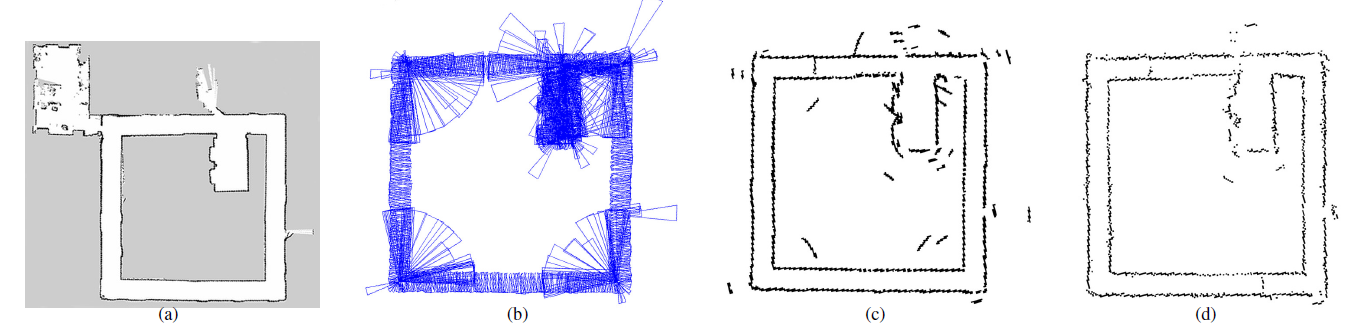
\includegraphics[width=1\linewidth]{Figures/Occupancy_Grid_Map/OGM_inverse_forward_compare}
	\caption{The experimental results from Carvalho's research \cite{carvalho2013comparative} which compares the inverse sensor model with the forward model. Figure (a) is the ground truth map. Figure (b) are the taken measurements. Figure (c) is the computed \gls{OGM} using the inverse sensor model. Figure (d) is the computed \gls{OGM} using the forward sensor model.}
	\label{fig:OGM_inv_for_comp}
\end{figure}

The forward sensor model is more accurate but also requires much more computational effort \cite{carvalho2013comparative}. Both probabilistic methods have in common that they cannot tell the difference between incompleteness (i.e. ignorance) and uncertainty. When the occurrence of an event does not hold absolute confidence, this lack of confidence can have two causes. The first cause could be that due to a lack of information another possible event is not excluded. This lack of information is defined as ignorance. A second cause could be that the occurrence of the event is not definitely true, which is defined as uncertainty \cite{liu2001propositional}.
The \glsfirst{DST} \cite{dempster1967upper} \cite{shafer1976mathematical}, however, can distinguish between ignorance and uncertainty. This theory can be used to generate better \glspl{OGM}. In the following subsection, evidential occupancy grid mapping, using the \gls{DST}, will be explained.


\subsection{Evidential Occupancy Grid Mapping} \label{subsec:evid_OGM}
In evidential Occupancy Grid Mapping, the \glsfirst{DST} is used to estimate the state of the occupancy grid cells. This method, as opposed to the probabilistic method, can distinguish ignorance (the cell is either empty or occupied) from uncertainty (there is evidence that the cell is both empty and occupied with a certain belief). However, more computational power is required for the evidential method compared to the probabilistic method \cite{moras2014evidential}. The following section will first explain the mathematics behind \gls{DST}. Then, its application on \glspl{OGM} is discussed. 


\subsubsection{The Dempster-Shafer Theory}
The DST formalizes the transferable belief model. The model defines a discrete \gls{FOD} which contains the set of possible states of a system. In the case of an \gls{OGM}, the \gls{FOD} is $\Omega = \{E, O\}$, with $E$ for Empty and $O$ for Occupied. A mass function $M$ is defined that maps the powerset $2^\Omega$ of $\Omega$ to the domain $[0 \; 1]$. The powerset is the set of all subsets of $\Omega$ including the empty set $\emptyset$ and itself ($2^\Omega = \{\emptyset, E, O, \Omega \}$). If $A$ is an element in $2^\Omega$, then $M(A)$ represents the amount of evidence (mass) that supports hypothesis $A$ within the domain $[0 \; 1]$. Then, two properties are set to the mass function $M$. First, $M(\emptyset) = 0$, and second, formula \ref{eqn:sum_massfunc} verifies that the sum of the masses of each hypothesis in the powerset is equal to $1$. This means that it is assumed that the powerset $2^\Omega$ is complete and that no evidence will be obtained that supports none of the hypotheses in the \gls{FOD}. A mass function with these two properties is called a \gls{BBA} mass function. \cite{moras2014evidential}. A \gls{BBA} mass function allows for the assignment of lower and upper bounds of a probability interval, belief $Bel()$ and plausibility $Pl()$ respectively, that represent the support to the hypotheses $A \in 2^\Omega$.

Belief is the sum of the masses of all the hypothesis's subsets including the hypothesis, as is shown in equation \ref{eqn:belief_func}, where $A$ and $B$ represent hypotheses (e.g. for the $\Omega$-hypothesis, this would be the mass of $\Omega$ and the subsets of $\Omega$: $E$ and $O$]).
In equation \ref{eqn:plaus_func} it can be seen that the plausibility is computed by taking $1$ minus the sum of the masses that exclude the hypothesis (e.g. for the hypothesis $O$, the plausibility $Pl(O)$ would be $1$ minus $M(\emptyset)$ and $M(E)$ which is $0.3$). \cite{moras2014evidential}.

\begin{equation} \label{eqn:sum_massfunc}
	\sum_{A \in 2^\Omega}^{} M(A) = 1 
\end{equation}

\begin{equation} \label{eqn:belief_func}
	Bel(A) = \sum_{B|B \subset A}^{} M(B) 
\end{equation}

\begin{equation} \label{eqn:plaus_func}
	Pl(A) = \sum_{B|B \cap A \not = \emptyset}^{} M(B) = 1 - \sum_{B|B \cap A = \emptyset}^{} M(B) 
\end{equation}

\hfill \break

An example of a \gls{BBA} mass function is shown in table \ref{tab:belief_func_example}, given the powerset $2^\Omega = \{\emptyset, E, O, \Omega \}$. In this example, a sensor reading obtains information that a certain grid cell is empty. The sensor reading's probability of being reliable is $0.7$ and $0.3$ for being unreliable. This information can be used to assign a subjective probability (mass) to each hypothesis, which sum up to $1$. A reliable sensor will give a true reading, so the hypothesis of the grid cell being empty ($m(E)$) is assigned a mass of $0.7$. However, given that there \textit{is} a grid cell ($m(\emptyset) = 0$), the sensor reading has a probability of $0.3$ that it is unreliable. This does not mean that the grid cell is occupied with a probability of $0.3$, but it means that it's state is uncertain with that probability. Therefore, a mass of $0.3$ is assigned to the hypothesis $m(\Omega)$ that states that the grid cell is either empty or occupied. The hypothesis of the cell being occupied ($m(O)$) will have a mass of $0$, since there is no evidence that supports it. \cite{shafer1992dempster}. Subsequently, the belief $Bel()$ and the plausibility $Pl()$ of the hypotheses are computed, giving the lower and upper probability bounds for the hypotheses. 


\begin{table}[h!]
	\begin{center}
		\caption{An example of a \gls{BBA} mass function.}
		\begin{tabular}{llll} 
			\toprule[0.25ex]
			Hypothesis & Mass & Belief & Plausibility \\ [0.5ex]
			\midrule 
			$M(\emptyset)$ & 0 & 0 & 0 \\ 
			$M(E)$ & 0.7 & 0.7 & 1.0 \\
			$M(O)$ & 0 & 0 & 0.3 \\
			$M(\Omega)$ & 0.3 & 1.0 & 1.0 \\
			\bottomrule[0.25ex]
		\end{tabular}	
		\label{tab:belief_func_example}
	\end{center}
\end{table}

\subsubsection{Applying \gls{DST} to generate \glspl{OGM}}
To generate an evidential \gls{OGM}, given independent sensor data, each grid cell is assigned a mass function $M_{i,j}$ with beliefs and plausibilities. If new sensor data about a grid cell is obtained, the DST method can fuse the mass functions of the current cell state and the new sensor data according to the joint mass equations \ref{eqn:fuse_dst} and \ref{eqn:conj_rule}. \cite{moras2014evidential}.

\begin{equation} \label{eqn:fuse_dst}
	M_1 \oplus M_2 (A) = \left \{ 
	\begin{array}{ll} 
	\frac{M_{1 \cap 2}(A)}{1 - M_{1 \cap 2}(\emptyset)} & A \not = \emptyset \\
	0	&	 A = \emptyset
	\end{array} \right \}
\end{equation}

Where $\cap$ is the conjunctive rule with $B$ and $C$ hypotheses and $A$ the joint hypothesis:

\begin{equation} \label{eqn:conj_rule}
	M_{1 \cap 2}(A) = \sum_{B, C \in 2^\Omega | A = B \cap C}^{} M_1(B) \cdot M_2(C)
\end{equation}

Then, a probability measure can be taken from the mass function according to equation \ref{eqn:belief_2_prob}. Here, $A$ and $B$ represent hypothesis subsets of powerset $2^\Omega$. The cardinality (number of elements in a subset) is denoted as two vertical bars $\vert \vert$.

\begin{equation} \label{eqn:belief_2_prob}
	P(A) = \sum_{B \in 2^\Omega}^{} M(B) \cdot \frac{\vert A \cap B \vert}{\vert B \vert}
\end{equation}

This equation is not bijective, meaning an infinite number of mass functions can be found given the same probability. This is because information that distinguishes ignorance from uncertainty is lost when the mass function is transformed to a probability. This lost information in probabilities is exactly what makes the DST method a more accurate but also a more computational method for \gls{OGM} generation. \cite{moras2014evidential}. The processing time of the DST method is about $1.5$ times higher than that of the inverse sensor model probabilistic method \cite{ribo2001comparison}. Figure \ref{fig:OGM_prob_DST_comp} shows the qualitative differences between the probabilistic approach (center) and the DST approach (right).  

\begin{figure}[h]
	\centering
	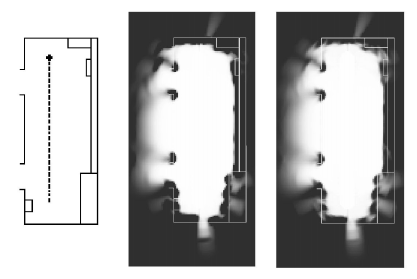
\includegraphics[width=0.6\linewidth]{Figures/Occupancy_Grid_Map/OGM_prob_l_DST_r_compare}
	\caption{Ribo and Pinz \cite{ribo2001comparison} compare the probabilistic method (center) with the DST method (right) to generate OGMs. The ground truth schematic is shown left.}
	\label{fig:OGM_prob_DST_comp}
\end{figure}

\newpage

\subsection{Alternative methods for Occupancy Grid Mapping} \label{subsec:alt_OGM}
Besides the probabilistic and evidential approach to generate \glspl{OGM}, there are more methods to determine which cells in the grid are occupied. Two methods, the possibilistic method and the \gls{NN} method are discussed in this section. These methods are less common than the probabilistic and evidential methods, therefore they are not explained in depth in this literature review. For more in depth information about the methods it is advised to read the papers from which the methods are cited. At the end of this section comparison methods of OGMs are discussed. 

\subsubsection{Possibilistic Occupancy Grid Mapping}
Oriolo \cite{oriolo1997fuzzy} defines the \gls{OGM} as two fuzzy sets where one set is empty ($E$) and the other occupied ($O$). Based on measurements, each cell is assigned a partial membership to states $E$ and $O$. This partial membership allows to process and distinguish insufficient (ignorance) from uncertain information. Ribo and Pinz \cite{ribo2001comparison} compare this fuzzy method (also called possibilistic) with the probabilistic and evidential methods and conclude that the possibilistic method is more conservative and thus more robust towards outliers compared to the other two methods. However, its robustness also causes loss of information and the emergence of artifacts. Like the DST method, the possibilistic method requires about $1.5$ times more computation time than the inverse sensor model probabilistic method. 

\subsubsection{\gls{NN}-based Occupancy Grid Mapping}
Thrun \cite{thrun1993exploration} uses an \glsfirst{NN} to generate an \gls{OGM} from measurements. In a simulated environment, the \gls{NN} is trained to interpret sensor data and estimate a confidence that a cell is occupied. This trained \gls{NN} is then tested in a real environment and shows it can model unknown environments efficiently, however the network cannot be trained until convergence because then it would overfit on the simulated environment and perform worse in real situations. Collins \cite{collins2007occupancy} compares the \gls{NN} method with the probabilistic method. The \gls{NN} method performs worse that the probabilistic one because it has a tendency to overestimate the free space beyond the actual environment borders. It also tends to model the sensor's extremities (maximum value due to no detection) as occupied areas, while the probabilistic approach's algorithm will ignore these extremities. Van Kempen \cite{van2021simulation} takes the use of \glspl{NN} to generate OGMs even further. Van Kempen proposes a deep inverse sensor model together with a PointPillars architecture (often used to process LiDAR data) extended with an evidential prediction head to estimate an evidential \gls{OGM}, including the uncertainties. The network is trained using a synthetic dataset. The network is then tested on synthetic data and on real-world data. It shows promising results on both synthetic data and real-world data. It performs better than classical approaches on the synthetic data, but the generalization capabilities are not sufficient yet to have accurate results on the real-world data. In future research, van Kempen suggests to use a more diverse dataset to train the network on for better generalization. 

\subsubsection{Comparison methods for \glspl{OGM}}
Metrics to measure and decide what \gls{OGM} generation method is the best are not easy to define. The computation time and memory requirements to generate the \gls{OGM} can be determined and used as a metric to compare efficiency of the \gls{OGM} methods. Most other methods to determine and compare the quality of \glspl{OGM} are qualitative (visual inspection) \cite{ribo2001comparison}. Collins \cite{collins2007occupancy} summarizes some quantitative metrics based on image similarity measures and one that bases the \gls{OGM} quality on the usefulness of the map for a robot to find paths, compared to the ground truth. More about metrics to evaluate \glspl{OGM} will be discussed in section \ref{sec:metrics}. \\

Besides ways to generate the traditional \gls{OGM} maps that provide information about the cell occupancy, there are extended \gls{OGM} forms that contain more information. The next subsections will elaborate on some of those extended forms.


\subsection{Occupancy Grid Map extended forms} \label{subsec:OGM_ext_form}
Many variations of the \gls{OGM} have been invented and researched that represent environments in more complex methods, including for example 3D information \cite{degerman20163d}, semantic segmentation of the cells \cite{lu2019monocular}, or dynamic information of the occupied regions \cite{nuss2018random}. 

\subsubsection{3D Occupancy Grid Mapping}
Degerman \cite{degerman20163d} proposes a way to create 3D Occupancy Grid Maps using 3D RADAR data. Degerman uses a binary Bayes filter to estimate the occupancy probabilities of the assumed independent voxels (grid cells in 3D). The RADAR data is obtained in spherical coordinates (radius $r$, scanning angle $\theta$, and azimuth angle $\phi$) after which those measurements are mapped to the Cartesian coordinates of the 3D \gls{OGM}. As shown in Figure \ref{fig:OGM3Dspherical}, the spherical measurement grid cells are dense in short range while the distances between them increase for longer ranges. Therefore trilinear interpolation is used to combine the spherical data points when they are mapped to the Cartesian coordinates. An example of the resulting 3D occupancy grid is shown in Figure \ref{fig:OGM3Dex}.


\begin{figure}[h]
	\centering
	\begin{subfigure}[t]{0.4\linewidth}
		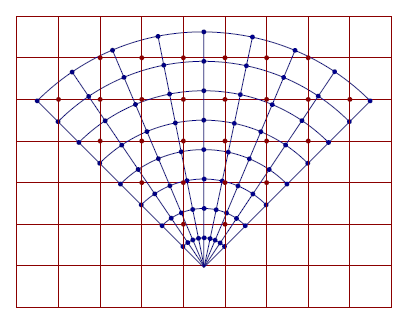
\includegraphics[width=1\linewidth]{Figures/Occupancy_Grid_Map/3D_Occupancy_Grid_Spherical_Coord}
		\caption{The 2D image of the measured spherical grid points (blue) and the Cartesian grid points that are computed by performing interpolation on the surrounding spherical points. \cite{degerman20163d}}
		\label{fig:OGM3Dspherical}
	\end{subfigure} \hspace{0.1\textwidth}
	\begin{subfigure}[t]{0.4\linewidth}
		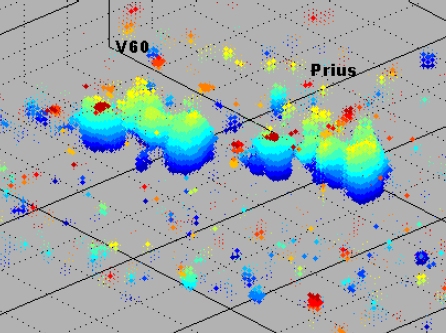
\includegraphics[width=1\linewidth]{Figures/Occupancy_Grid_Map/3D_Occupancy_Grid_example}
		\caption{An example of a 3D occupancy grid where each voxel with a likelihood value above a certain threshold is visualized. The blue color represents lower levels while the red color represents higher levels. The clusters of occupied voxels represent two cars (V60 and Prius). \cite{degerman20163d}}
		\label{fig:OGM3Dex}
	\end{subfigure}
	\label{fig:OGM3Dboth}
\end{figure}




\subsubsection{Semantic Occupancy Grid Mapping}
While classical OGMs only contain information about occupancy, Lu \cite{lu2019monocular} proposes a method that utilizes the semantics of the environment in an \gls{OGM}. The method they propose is an end-to-end convolutional neural network with a variational autoencoder-decoder part that takes monocular RGB camera data as input and outputs an \gls{OGM} with an additional semantics channel. They distinguish the environment with four labels: road, sidewalk, terrain, non-free space. The network is trained and evaluated on the Cityscapes \cite{cordts2016cityscapes} and KITTI \cite{geiger2013vision} datasets and the results show that the network is robust to sparse input data and a weak ground-truth. Figure \ref{fig:sem_OGM} shows an illustration of the semantic \gls{OGM} method.

\begin{figure}[h]
	\centering
	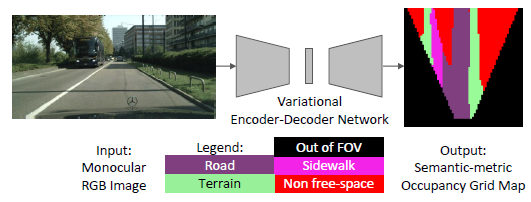
\includegraphics[width=0.7\linewidth]{Figures/Occupancy_Grid_Map/Semantic_OGM_Network}
	\caption{An illustration of the semantic \gls{OGM} method that takes a monocular RGB image as input and outputs a semantic \gls{OGM} \cite{lu2019monocular}.}
	\label{fig:sem_OGM}
\end{figure}


\subsubsection{Dynamic Occupancy Grid Mapping}
Besides having information about semantics in an \gls{OGM}, for purposes such as motion planning and tracking, information about the environment's dynamics is also desired. 
Danescu \cite{danescu2011modeling} proposes a particle based method for tracking the dynamic driving environment in occupancy grids. This method represents the world as a 2D BEV grid in which each obstacle is represented by a set of particles that are located in the grid's cells. Each particle has their own position and speed and can move between cells based on their dynamics. Also, particles can be created or destroyed over time. The occupancy probability of a cell $C$ is estimated by the ratio of the number of particles in that cell and the total number of particles allowed for a single cell $N_C$.
The number of particles allowed for a single cell is predetermined, while the total number of particles in the grid, $N_S$ is not fixed and is dependent on the number of obstacles in the environment.
By taking the average speed of all particles within a grid cell, the speed estimation of that cell is estimated. If obstacles in the environment overlap, the particles in a single cell can have different speeds. Clustering of the speeds can be used to model the speeds of multiple obstacles that overlap in a cell. This way, a tracking algorithm is used to create, update, and destroy particles to estimate the occupancy and dynamic state of the real world. These states generally are saved in separate channels of the grid, one for the occupacy state, and two for the speed and orientation of the grid cells. \\

Nuss \cite{nuss2018random} continues this research and proposes an improved method, using the Dempster-Shafer theory, to assign particles to grid cells. They name this method the Dynamic Occupancy Grid Map (DOGMa). An example is shown in figure \ref{fig:DOGMa_example}.

\begin{figure}[h]
	\centering
	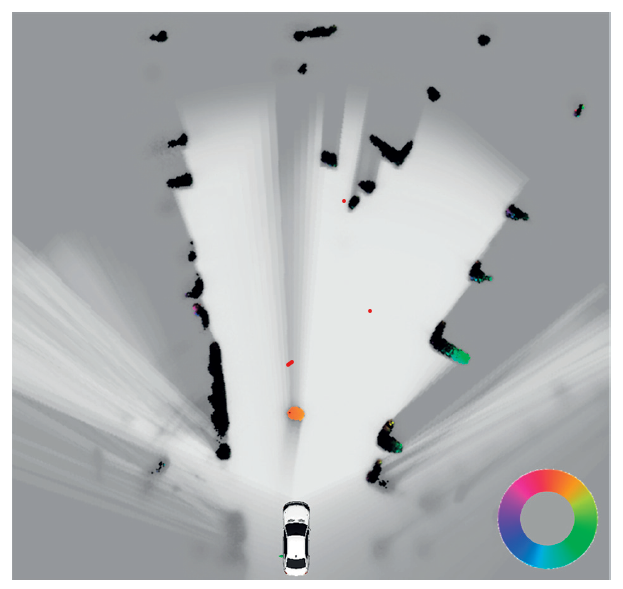
\includegraphics[width=0.4\linewidth]{Figures/Occupancy_Grid_Map/DOGMa_example}
	\caption{A Dynamic Occupancy Grid Map example in which the static parts (occupancy information) are shown in black and white, with black occupied and white emtpy space. The dynamic information is shown in color. The color code represents the direction of the grid cell corresponding to the color wheel at the bottom right. The saturation value of the color determines the velocity, where the velocity is higher if the saturation is higher. \cite{nuss2018random}.}
	\label{fig:DOGMa_example}
\end{figure}

Besides the 3D \gls{OGM}, semantic \gls{OGM} and the DOGMa, there are more variations to occupancy grid maps. In some papers, the term \gls{OGM} is not used however, making it sometimes hard to define what is still an \gls{OGM} and what isn't. 
For example, Wu \cite{wu2020motionnet} proposes a method to predict future environments using Bird's Eye View (BEV) maps. The paper states that they define an alternative to OGMs, which they call a BEV map. The BEV map is a grid map with discrete occupancy information in each cell. The BEV map has multiple channels. Each channel represents another height layer of the environment, which basically means that the whole BEV map is a 2D pseudo-image, because all layers together form a 3D representation of the environment. In principle, this approach is similar to a 3D \gls{OGM}. In Wu's method, a Deep Learning Network is used to apply semantics to the BEV map and estimate temporal features (the dynamics). In essence, Wu's method creates OGMs that are 3D and incorporate semantics and dynamics. In this literature review, environment representations such as Wu's are also considered \gls{OGM} variations. \\

\subsection{What OGM form is most suitable to use in OGM prediction methods?} \label{subsec:OGM_conclude}

What \gls{OGM} form is best depends on the requirements of the prediction method. Table \ref{tab:ogm_overview} shows an overview of the different \gls{OGM} generation methods. In the case of \glspl{AV}, there will be a trade-off between accuracy and computation time. If a fast method is desired, the inverse probabilistic method would be the best choice. The downside is that the accuracy will be lower compared to most other methods and there is no distinction between ignorance and uncertainty. If a higher accuracy is desired and there is the means to carry a higher computational load, the \gls{DST} or possibilistic generation methods are more suitable because of their high accuracy and distinction of ignorance and uncertainty. The possibilistic method is more conservative than the \gls{DST} method, which results in fewer outliers but more artifacts and information loss in the \glspl{OGM} compared to the \gls{DST} method. In the context of \glspl{AV}, having artifacts in the \glspl{OGM} and a higher information loss both might result in dangerous situations in which the \gls{AV} either perceives something that is not present, or does not perceive something that is present. Therefore, the best option would be the \gls{DST} method. Due to the high computational effort of the forward sensor model, and because the \gls{NN}-based method is not developed enough to acquire a good accuracy in real situations, these options are considered the least suitable for \gls{OGM} prediction purposes. 	 


\begin{table}[h!] 
	\caption{This table gives an overview of the properties of each \gls{OGM} generation method based on the information in this chapter.}
	\centering
	\resizebox{\linewidth}{!}{%
		\begin{tabular}{llll} 
			\toprule[0.25ex]
			& \textbf{Accuracy} & \textbf{Computation Effort} & \textbf{Ignorance-Uncertainty Distinction} \\ 
			\midrule
			\textbf{Inverse Probabilistic} & Average & Low & No \\
			\textbf{Forward Probabilistic} & High & High & No \\
			\textbf{\gls{DST}} & High & Average & Yes \\
			\textbf{Possibilistic} & High & Average & Yes \\
			\textbf{Neural Network Based} & Low & Unknown & Yes \\
			\bottomrule[0.25ex]
		\end{tabular}
	}
\label{tab:ogm_overview}
\end{table}

Further, regarding the extended forms, each extension will provide the \gls{OGM} with more information. Generally, when performing predictions, having more information will result in better predictions. The trade-off in this case is again one of accuracy versus computation effort. Whether the amount of additional information is worth the additional computation effort depends on the goal of the predictions. \\

The next section will discuss the available datasets that are used to obtain Occupancy Grid Maps from for research and what metrics are used to determine the accuracy of those OGMs. 

